\chapter{引言}
\label{cha:intro}

\section{故障诊断的研究背景及意义}

当前,随着德国“工业4.0”及美国“工业互联网”计划席卷全球,世界正式揭开了
第四次工业革命的序幕。为了提高本国的工业竞争力,世界各国相继提出了自己
的“工业4.0计划”。中国作为世界第一制造大国,强烈地喊出了“中国制造2025”
计划,这是我国从世界大国转向世界强国的顶层设计,这一计划涉及到了许多高
科技复杂系统的制造,比如航空航天装备、高档数控机床和机器人、轨道交通装
备等等。在轨道交通方面,当前我国已拥有世界上最先进的高铁技术和最长的通
车里程,达到18000公里,区域网覆盖了中国绝大多数的城市。但是,无论是高铁
动车技术、还是航空航天装备,我们都无法忽视这些复杂系统背后一直存在的重
大问题——故障。同样以高铁为例,因为高速列车运行时速极高,任何微小的故障
或隐患若不能及时的诊断并有效处理,都导致难以想象的后果,造成无法弥补的
损失,严重影响政治、经济、社会的和谐发展。

1998年6月,德国高速列车轮箍的金属疲劳,轮箍发生断裂,导致列车出轨死亡
100多人。2011年7月23日,温甬线特大交通事故造成40人死亡,172人受伤,原
因是列控中心设备存在严重缺陷,设备发生故障后应急处理不到位。航空航天领
域更是故障发生的重灾区。美国挑战者号航天飞机升空不到两分钟即发生爆炸,
机上所有宇航员不幸遇难,这次事故对美国航天事业产生严重的影响,一度使其
停滞不前, 原因是固态火箭的右侧的推进器上的一个O形环发生故障从而失效,
随后出现了连锁反应。1986年4月,前苏联的切尔诺贝利核电厂的4号反应堆发生
爆炸,导致严重的核泄漏,近几十年来因受核辐射影响累计死亡人数达9.3万人,
直接经济损失180亿。1984年12月印度的博帕尔毒气泄漏事故造成2.5万人直接致
死,55万人间接致死,另外还有20多万人永久残废的人间惨剧。这些惨痛的教训
警示着人类,及时发现工业系统设备的故障,保障工业系统设备的健康正常运行
具有举足轻重的地位。发现并检测故障,进行故障诊断和有效的处理防护,这在
工业系统中是必不可少的一环。因此,在“中国制造2025”,“十三五”规划的战略
背景下,在推动我国高端技术产业大步发展的同时,必须高度重视这些高端复杂
设备系统背后频繁出现的故障问题,认真研究先进的故障诊断技术,及时发现故
障并做有效处理,为我国高端设备制造业的发展保驾护航。

\section{故障诊断国内外研究现状}

\subsection{概述}

许多的工程系统包括航空航天设备、化工系统、高精度数控机床、电力网络等等
对系统的安全稳定运行要求很高。随着系统潜在可能的故障增多以及设备本身的
经济成本增加,人们对系统的的安全性和可靠性的要求也越来越高。因此有必要
尽可能地诊断出潜在的故障并及时有效处理,避免出现危险情况,保证系统的有
效运行。文献~\inlinecite{van1997remarks}指出故障是正常运行系统的部分参数或者
状态性能出现了与期望不相符的偏差。比如执行器锁死、传感器失效或者系统部
件连接中断等等均属故障。一般来说,故障分为系统故障、执行器故障和传感器
故障。系统出现故障会造成系统控制器的信号无法正常到达执行器或直接影响系
统的输入输出性能,执行器出现故障会使得执行器无法有效完成控制器下达的控
制指令要求,传感器故障会产生系统状态测量误差。

在对系统的监测过程中,一个故障诊断系统需要能够完成对被测对象发生的故障
进行告警,确定故障发生的位置以及估计出故障发生的严重程度。因此,可将故
障诊断需要完成的任务分解为以下三个方面:

1)故障检测(Fault Detection):确定系统是否发生了故障。

2)故障隔离(Fault Isolation):在故障检测阶段确认系统发生故障之后,进
一步确定故障的种类以及故障发生的位置。

3)故障识别(Fault Identification):在完成故障隔离步骤之后,估计故障发
生的严重程度。故障检测对于任何一个系统都是至关重要的一步,是完成故障诊
断其他任务的基础环节;故障隔离为维修人员提供辅助帮助,可以极大的提升系
统设备的维修效率;故障识别为维修人员采取何种维修手段提供了重要的依据。

为了提高系统的可靠性,
通常采用硬件冗余或者软件冗余(也称分析冗余)的方式,对故障进行检测、
隔离和识别。硬件冗余采用多套系统进行备份,当前运行系统被判定已经故障之
后,就切换到其他正常的备份系统。但硬件冗余的代价太高,经济成本很大,再
者由于空间或者重量的限制,对其物理安装也提出了挑战。随着现代控制理论的
发展,从20世纪80年代以来,分析冗余技术已成为了故障诊断技术的主流技术。
相比于硬件冗余技术,分析冗余诊断方法的效率更高,但由于环境噪声、模型及
数据误差、系统性能和控制策略的复杂性等因素的影响,分析冗余技术在实际应
用中面临着更多的挑战。总之,故障的位置、大小、类型等信息对系统采取及时
的容错策略保证系统的正常运行是具有重要意义的。

在本课题的调研过程中,将目前现有的故障诊断方法大致分为两类:基于模型的
故障诊断方法以及基于数据的故障诊断方法。各类故障诊断方法对照此分类规则
的分类结果图如图~\ref{fig:method_summary}所示。
\begin{figure}[ht]
  \centering
  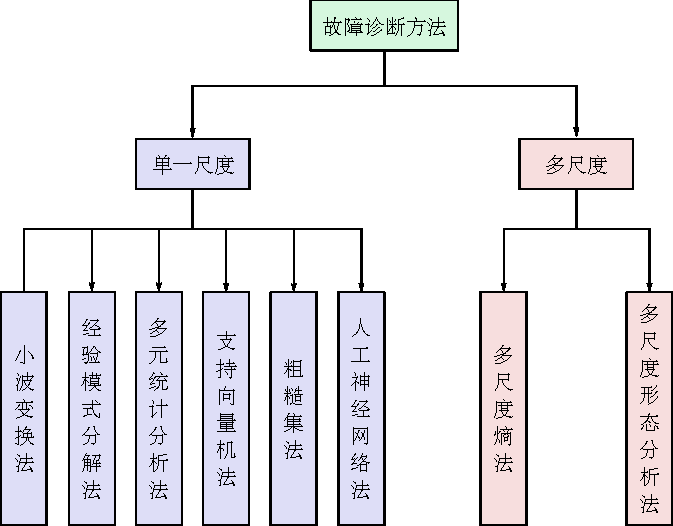
\includegraphics{method_summary}
  \caption{常见的故障诊断方法分类}
  \label{fig:method_summary}
\end{figure}

\subsection{基于模型的故障诊断方法}

基于模型的故障诊断方法是指利用系统的结构、行为和功能等方面的知识对系统
进行诊断推理,在进行推理之前需要建立系统的结构、行为或功能模型。文献~\inlinecite{davis1984diagnostic}
提出的“基于结构与行为的诊断推理”以及~\inlinecite{reiter1987theory}发表
的“基于第一定律的诊断理论”奠定了基于模型的故障诊断的理论体系。之后,
威廉姆斯对系统的定性模型建立方法及基于模型的推理算法进行了深入的研究,
取得了极大的研究成果~\cite{hofbaur2004hybrid, hofbaur2002hybrid}。

基于模型诊断的基本思想就是,利用系统内部结构、行为或者功能模型来预测系
统行为,并将这些模型预测值与系统观测值进行比较~\cite{console1999model, davis1988model, mosterman1998comprehensive}。
如果预测值与观测值一致,则说明系统工作正常;如果存在差异,则利用这些差
异来搜索那些可使预测模型与观测值相一致的各种可能行为的状态假设,这些状
态假设就是基于模型的故障诊断方法中所得出的诊断结果~\cite{wotawa2000debugging, friedrich1999model}。

从建模的角度看,基于模型的方法包括定量模型(精确数学模型)、半定量模型
和定性模型方法。定性方法不同于定量方法的地方在于:

1)物理量尺度不同

在定量方法中,物理量用精确的数值表示,而在定性方法中,物理量的尺度是被
路标值离散化的实空间。

2)物理模型不同

定量方法中使用的是定量物理模型,物理量之间的关系用代数方程、微分方程等
精确描述,系统的因果关系必须在模型外由人来给出。而在定性方法中使用的是
定性物理模型,物理量之间的关系用定性约束,系统的前后因果关系体现在模型
之中。

3)求解过程和所得结果不同

在定量的方法中,求解的过程就是求解代数方程或微分方程的过程,最后得到的
结果是精确的物理量数值。而在定性的方法中,求解的过程是一个局部传播推导
的过程,最后获得结果是系统的行为描述,可以对系统的行为进行预测和解释。

4)推理能力不同

定量的诊断方法中,物理量之间的关系都是精确描述的,模型本身不具备推理能
力,系统的行为分析和因果解释由人来最后完成。而在定性方法中,因果关系直
接反映在系统的结构描述中,在求解的过程中就能够实现对系统行为的预测和解
释。

\subsubsection{定量模型的故障诊断方法}

基于定量模型的故障诊断方法也叫基于解析模型的诊断方法,其核心思想是用解
析冗余代替硬件冗余,以系统的数学模型为基础,利用观测器、等价空间方程、
卡尔曼滤波器、参数模型估计和辨识等方法产生残差,然后基于某种准则或阈值
对该残差进行评价和决策~\cite{raghuraj2008variable, twellmann2008model, rodrigues2008fault}。
目前常用的技术方法有:

1)状态估计法

状态估计法是用真实系统的输出与观测器或滤波器的输出进行比较形成残差~\cite{gao2006kalman, qian2001digital, piatyszek2000fault}。
如图~\ref{fig:state_estimation}所示,当系统正常工作时,残差为零,发生
故障时,残差非零。从残差中提取故障特征,并设计相应的判决分离算法实现故
障诊断。状态估计常用的方法有:故障检测滤波器方法和卡尔曼滤波器方法等~\cite{goel2000fault}。
普尼特等人提出了一种基于多卡尔曼滤波器的故障检测和辨识方法,自适应的调
整滤波器去预测可能出现的故障类型。当预报读数和实际传感器读数不同时,这
个残差就作为每个滤波器的工作状态的指示器。
\begin{figure}[ht]
  \centering
  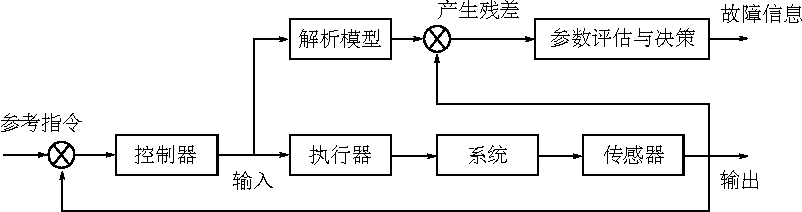
\includegraphics{state_estimation}
  \caption{状态估计法}
  \label{fig:state_estimation}
\end{figure}

2)参数估计法

参数估计方法通过对系统模型参数的辨识来达到目的,即由参数的显著变化来描
述故障,基本思想就是把理论建模与参数辨识结合起来,根据参数变化的统计特
性来检测故障信息,根据参数估计值与正常值之间的偏差来判断故障的情况。

故障诊断的参数估计方法主要有强跟踪滤波器方法,其最大特点就是利用了强跟
踪滤波器估计模型参数,强跟踪滤波器对不确定性模型具有鲁棒性,对突变和缓
变状态有很强的跟踪能力。针对实际系统中存在的随机噪声,Juricic等人结合
数理统计方法设计了随机系统的参数估计故障诊断方法,并具有一定的鲁棒性~\cite{jurivcic2002robust}。
在~\inlinecite{yu1997fault}中研究人员将参数估计法和观测器法相结合,构
造故障检测观测器,快速检测故障并进行故障预分离,再基于包含可能故障的简
化模型作参数估计,进一步实现故障分离。

状态估计法具有较好的实时性,因为不论是常规的观测器还是卡尔曼滤波器都是
呈指数型收敛的,这在实际应用中有很大的价值,而参数估计法的收敛性要差一
些,会导致比较大的延时。状态估计法对系统输入信号的要求不是很严格,并不
需要有连续不间断的激励信号的存在,而参数估计法却总需要有激励信号存在,
这一点也限制了参数估计法在实际中的应用。为了准确诊断,Qinghua Zhang于
2001年提出了一种新的适应观测器的设计方法~\cite{zhang2002adaptive},综
合应用了状态估计法和参数估计法,特别适用于多输入多输出线性时变系统。 

3)等价空间法

等价空间法的实质是把测量信息进行分类,得到最一致的冗余数据子集,用于系
统的状态估计,并识别出最不一致的冗余数据,即可能发生故障的数据。等价方
程法是一种无阈值的方法,需要较多的冗余信号,因此当被测量过程个数较多时,
计算量会显著增大。这种方法特别适于维数较低的被测量的冗余信号的优劣判别,
因为这类系统通常拥有较多的冗余测量信号,以提高控制系统的可靠性。Medvedev
提出了采用伪微分算子的等价空间法~\cite{medvedev1997disturbance},进行
故障检测和识别,并把这种方法应用到回旋式滑窗中,分析表明这种等价空间法
能达到很好的性能~\cite{magni1994residual}。

\subsubsection{定性模型的故障诊断方法}

美国德州大学的Kuipers较早进行定性建模和定性仿真工作,他于1986年在人工智
能杂志上发表了题为“定性仿真”的论文~\cite{kuipers1986qualitative},为定性
建模和定性仿真奠定了很好的研究与应用基础。Kuipers的方法总结了前人的思想,
并以严格的形式定义了定性仿真的算法。它是一种面向约束的方法,从一个定性约
束集和一个初始状态出发,预测系统未来所有可能的行为,作为微分方程的抽象,
定性仿真有着精确的数学语义。系统的定性仿真是从已知的系统结构和一个初始状
态出发,产生一个有向图。该有向图由系统未来可能的状态和状态之间的直接后继
关系组成,系统的行为就是有向图中从初始状态出发的一条路径\cite{forbus1984qualitative, forbus1991qualitative, williams1991qualitative}。

定性模型方法可分为因果图法、故障树法和定性物理法。基于模型的推理从机制的
定性描述和初始状态出发,产生可能行为的定性描述。一种利用定性推理完成故障
诊断的框图如图~\ref{fig:qualitative_reasoning}所示。
\begin{figure}[ht]
  \centering
  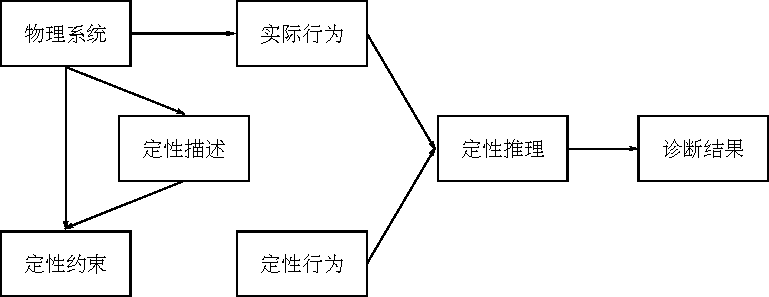
\includegraphics{qualitative_reasoning}
  \caption{基于模型的定性推理故障诊断方法示意图}
  \label{fig:qualitative_reasoning}
\end{figure}

1)因果图法 

定性方法中引入因果关系,主要是为了定性解释,即通过推理步骤来解释行为,并
且主要是状态间行为。引入因果关系的好处在于:首先,其描述了系统如何产生其
行为,说明了系统部件间的作用,可直接用于诊断。其次,利用因果关系可以揭示
系统行为的更多信息。最后,因果关系作为一种系统理解的通用性模式,可用来解
释系统。系统间的因果关系可描述为有向图SDG的形式~\cite{forbus1984qualitative, forbus1991qualitative, williams1991qualitative},
节点间的有向边表示由原因节点到结果节点。SDG为图形化描述定性模型提供了非常
有效的方法~\cite{tarifa2004fault},已经大量用于故障诊断中。Ir等最先把SDG
用于故障诊断中,并总结出了因果图~\cite{zhang2005sdg}。Umeda总结了如何从系
统的微分代数公式中得到SDG~\cite{umeda1980graphical};Shiozaki解决了SDG描
述中的条件依赖性问题~\cite{shiozaki1985fault}。利用SDG的基于规则的方法也
由Kramer引入到故障诊断中~\cite{kramer1987rule}。

2)定性物理法

故障诊断中的定性物理方法可分为两类,第一类就是由微分方程推理出定性方程,
Kleer在系统定性建模和因果知识描述领域已经做了相当大的工作~\cite{de1992characterizing, de1987diagnosing, de1984qualitative}。
定性物理中的其它方法是从普通微分方程ODE中推理出定性行为,许多不同故障的
定性行为可用作知识源。基于模型诊断的应用中最有代表性的就是NASA的DS-1中采
用的Livingstone~\cite{schwabacher2002nasa, bernard1998design}系统,它是
一个基于模型的诊断系统,与自主规划器和执行器相结合,可实现系统的在线自主
诊断和重配置。Livingstone采用命题逻辑语言来描述模型~\cite{muscettola1998remote, williams1996model},
把组件描述为有限状态机~\cite{williams1996autonomous, genc2007distributed}而扩
展了基于模型诊断的思想。

\subsection{基于数据的故障诊断方法}

本课题将基于数据的故障诊断方法在诊断过程中是否需要故障类别信息划分为基于
数据的有监督的故障诊断方法以及基于数据的无监督的故障诊断方法。

其中,基于数据的有监督的故障诊断方法可大致划分为基于信号处理的故障诊断方
法,基于数据知识的故障诊断方法,基于统计分析的故障诊断方法三类。基于数据
的无监督的故障诊断方法主要是相关的异常检测方法。

\subsubsection{基于数据的有监督的故障诊断方法}

基于数据的有监督的故障诊断方法主要分为三类:基于信号处理的方法、基于统计
分析的方法和基于数据知识的方法。

基于信号处理的故障诊断方法基本思想是:利用信号处理的方法对收集到的信号进
行分析处理,提取信号特征,对比已有的故障信号特征,从而达到诊断出系统故障
的目的,目前常用的基于信号处理的故障诊断方法主要有小波变换法、经验模式分
解法、形态信号处理法以及谱分析法。

1)小波变换法

基于小波变换方法实现故障诊断的基本思想是:在时频域,利用小波变换的方法对
原始信号进行多尺度多分辨率的细化分析,从而提取信号的特征信息完成故障诊断~\cite{naderi2008modeling, carneiro2008incipient}。

小波变换是一种可用于非平稳、时变信号的时频局部分析技术,由短时傅里叶变换
发展而来,通过伸缩和平移等运算功能对信号进行多尺度的细化分析。小波变换克
服了短时傅里叶变换无法同时兼顾良好频率和时间分辨率的缺陷,在时域和频域均
可以表征信号局部特征。其时间窗和频率窗大小都可以改变,在低频部分具有较高
的频率分辨率和较低的时间分辨率;在高频部分则具有较高的时间分辨率和较低的
频率分辨率~\cite{zhoudonghua2009fault}。小波分析变换的这种性质可以使得我
们能够分辨出原始信号某时刻的瞬态特征,而且能保留信号的主要频域成分,从而
达到滤波噪声的效果。文献~\inlinecite{misra2002multivariate}利用小波变换对
信号进行多尺度分析,提取信号在不同尺度上的特征用于故障诊断。文献~\inlinecite{stoianov2001wavelet}
将小波变换技术用于管道系统泄露检测中,选择特殊的小波系数,从而检测并定位
出泄露。文献~\inlinecite{aminian2000neural, abbasion2007rolling, lou2004bearing}
中,研究人员们将小波变换与人工神经网络、支持向量机、模糊逻辑等其他方法相
结合,进行故障检测和分类。

文献~\inlinecite{riera2008general}基于电流频率滑动预处理和离散小波变换,
诊断出了在速度和故障变化情况下的定子和转子故障。该文利用不同分辨率下小波
信号的平均功率计算作为一个动态故障指示器以量化故障程度。由于地下电缆的大
部分早期故障是由电缆绝缘失效、电缆连接处或者其他配件缺陷所导致,这类故障
反复发生,最终会变为永久性故障。为此,文献~\inlinecite{sidhu2010detection}
提出用小波变换和电流分析两种算法检测和分类不同电压等级下的地下电缆的早期
故障。其中,一种算法基于小波分析,用于检测由故障导致的瞬态过程,从而识别
早期故障;另一种算法基于对时域中的叠加故障电流和负序电流的分析,实现了对
单相对地故障的检测。

由于小波变换具有多分辨率特征,使其有力地克服了传统傅立叶变换在时域和频域
均具有较高的局部性的缺点,因此目前在非线性、非平稳信号分析中是较为常用的
时频域分析工具~\cite{junsheng2007application},能有效识别故障信号,达到
故障诊断的目的。此外,小波变换具有多尺度性和“数学显微镜”特性,这些特性使
得小波分析能识别振动信号中的突变信号~\cite{wang1996application},因此目前
运用小波变换法对微小故障进行诊断的研究和应用较多。但小波变换由于基函数长
度有限,小波谱的时间和频率分辨率是相互影响的,对信号做小波变换会产生能量
泄漏,从而影响分辨率,且变换结果依赖小波基的选择和分解尺度,自适应性不强~\cite{doudongyang2010ensemble}。

2)经验模式分解法

经验模式分解法(empirical mode decomposition, EMD)实现故障诊断的基本思
想是:假设任何信号都是由不同的本征模态函数(intrinisic mode function, IMF)
组成,每个IMF可以是线性的也可以是非线性的,表示了信号的内在特征振动形式。
其本质是通过特征时间尺度获得信号的本征振动模式,然后利用本征振动模式不断
地“筛”信号,从而诊断出故障~\cite{lei2013review}。

文献~\inlinecite{luozhonghui2005study}提出用EMD法诊断电机轴承内圈损伤早期
故障。由于机器运转时的背景噪声一般较大,特征信息常常淹没在背景噪声中不易被
识别出来,故该文先用小波变换对采集的电机轴承振动信号进行信噪分离,然后通过
EMD法将提纯的信号分解而得到若干个IMF,利用IMF的频谱突显轴承早期故障的特征
信息。由于EMD处理的是一维的信号,无法实现信息的融合,为此文献~\cite{yang2011bivariate}
用二元经验模式分解法检测风轮机中感应电机转子电气不平衡早期微小故障,并指
出该方法在检测变速机械的早期故障时比传统的基于EMD的方法和基于小波的“能量
跟踪”更为有效。

EMD由于有完全自适应能力而使其具有较好的处理非平稳和非线性信号的能力, 但
EMD算法本身也存在一些不足, 如均值与停止条件、端点效应、模式混淆等~\cite{doudongyang2010ensemble},
因而出现了一些改进的EMD方法, 但这些改进都是针对特定情形而进行的。

3)形态信号处理法

形态信号处理法(morphological signal processing, MSP)是一种非线性的时域
空间上的信号处理方法,要包含腐蚀、膨胀、开运算和闭运算四算法。利用MSP进
行故障诊断的主要思想是:过一个设计的“探针”(结构元素)在信号中不断移动,
寻找有物理意义信号之间的相互联系,取有用的信息从而诊断故障。文献~\inlinecite{he2010joint}
中提出使用MSP提取旋转机械故障诊断信号的弱周期性脉冲。该文首先使用小波滤
波器消除噪声干扰以增强脉冲特征,然后通过形态的闭合算子和局部最大算法处理
滤波后的信号,提取周期性脉冲。

MSP对信号的局部几何特征具有良好的敏感性,并且能够高效地处理脉冲信号。但该
方法也存在着一定的不足,当噪声过强以至于由于故障产生的脉冲完全被噪声淹没
时,依赖于信号形状的MSP性能将被破坏;另外由于需要有关信号的先验知识去定义
扁平结构元素的长度,因此该方法缺乏自适应能力。因此在故障诊断领域的应用范
围有限。

4)谱分析法

谱分析法的基本思想是:由于不同类型的故障会导致测量信号的频谱表现出不同的
特征, 故可通过对信号的功率谱、倒频谱、高阶谱等进行谱分析的方法来进行故障
诊断~\cite{liuxuexia2008high, yu2005application},因此文献~\inlinecite{drago1979incipient}
最早提出将谱分析的方法用于诊断旋转机械的早期故障。而文献~\inlinecite{garcia2011robust}
首先用快速傅里叶变换提取电机线电流的频谱,然后将小波函数的多分辨率技术应
用到电机线电流的频谱中,以便检测重要的峰值以及测量这些峰值相对于“基准”信
号的高度,最后基于鲁棒多元控制图进行转子断条故障的早期检测。由于基于傅里
叶的方法的时变特性使得它们不适用于非线性和非平稳系统的分析,文献~\inlinecite{he2010joint}
提出了结合小波包技术的多维谱分析方法,以辨识故障源并对非平稳振动的微小故
障信号进行早期检测。由于高阶谱对高斯有色噪声不仅具有很好的噪声抑制能力, 
而且能保持非线性系统的相位信息, 文献~\inlinecite{oh2006advanced}利用高阶
谱分析技术提取了滚动轴承的滚动体、内圈和外圈表面局部点蚀3种典型早期故障
信号的特征。考虑到与故障有关的频谱成份的幅值与频率随着电机负载的变化而变
化,文献~\inlinecite{gazzana2010system}提出了电机电流特征分析(motor 
current signature analysis method,MCSA)法进行电机中常见早期故障的诊断。
该文通过MCSA检测电机电流的频谱以检测与故障相关的特定成分, 然后基于这些成
分的相对振幅诊断故障, 从而有效地诊断出了电机中常见的几个早期故障(转子断条、
定子绕组短路和气隙偏心),并将其应用在在巴西南部的热电站中。为了区分不平
衡负载和绕组故障,文献~\inlinecite{oliveira2011power}通过对带载激励电流扩
展Park矢量模的交流成分进行频谱分析,从而诊断出三相电力变压器绕组的匝间短
路早期故障。

由于Duffing振子的相变对于和参考信号有微小角频率差别的周期性弱信号很敏感,
故间歇混沌弱信号检测方法被用于早期故障检测,但其中的一个重要的问题是如何
确定故障的特征频率。为此,文献~\inlinecite{xiong2007direct}提出混沌振子阵
列法检测往复阀的早期故障。但是如果混沌振子阵列法得到的频带很宽,大量的混
沌振子会被包括,从而使得计算更为复杂,因而文献~\inlinecite{zhao2009intermittent}
应用倒谱分析法确定微弱故障信号的特征频率,通过这个特征频率计算参考信号的
角频率,然后通过引入一个Lyapunov指数实现了对液压管测试仪中的往复阀的早期
故障的检测。

由于故障会引起频谱表现出不同的特征,故谱分析法被广泛地用于检测早期故障。
但是传统谱分析方法是以傅里叶变换为核心的,因此提取平稳信号特征效果较好,
但实际系统发生故障后的测量信号往往是非平稳的,即使使用短时傅里叶变换将
非平稳信号分为短的伪平稳段,基于傅里叶变换的方法也不适合复杂时频特性的
分析,这些都是用谱分析方法进行微小故障诊断时需要考虑的问题。

统计分析方法是一种将历史数据加以统计分析的方法,目前常用的主要有多元统
计法以及时间序列法。

1)多元统计分析法

基于多元分析的故障诊断方法的基本思想是:根据过程变量的历史数据,利用多
元投影方法将多变量样本空间分解,并在子空间中构造能够反映空间变换的统计
量,利用计算出的统计量指标以检测设备运行过程中变化的故障,基于多元统计
分析的故障诊断方法主要有主要分析法(principal component analysis,PCA)~\cite{zhao2008line}
和指定元分析法(designated component analysis,DCA)~\cite{zhou2008dca}。

PCA技术~\cite{abdi2010principal}强系统高维历史数据组成矩阵,进行一系列
矩阵运算后确定若干正交向量,历史数据在这些向量上的投影反映数据变化最大
的几个方向,舍去数据变化较小的方向,由此可将高维数据降维表示,经由PCA
技术降维后,通常只需要2~3维即可反映历史数据的大部分变换方向,进而从海量
数据中抓住主要部分,极大简化数据利用。

运用PCA技术进行故障定位经典的方法是贡献图法~\cite{miller1998contribution},
当判断发生故障时,定义故障贡献度函数,分别计算多个变量的贡献度函数值,
并选取使函数最大的变量作为引起故障的变量。PCA技术用于故障分类的原理是
以包含各类故障信息的数据为训练数据,推导出指示数据变化最大的几个方向的
向量。将新观测的数据代入预先定义的故障分类判别式中,通常采用模式分类方
法中的后验判别式~\cite{duda2000pattern},依据达到最大的故障概率来对故障
进行归类。文献~\inlinecite{raich1996statistical}提出了以每类故障为训练
数据分别建立PCA模型,依次对新观测数据进行检验以确定属于哪种故障数据或新
的故障类。

由于PCA方法能检测出缓变的信号,文献~\inlinecite{gezhiqiang2007mewma}利
用PCA方法检测焚烧炉的早期故障,并设计出一个软件包,专门用于检测都市固体
废物焚烧炉(municipal solid waste incinerators, MSWIs)中的3种早期故障
–—局部烧穿、局部焦化和排渣故障,并已将其用于实际生产。为了解决过程变量
之间具有相关性的微小故障的诊断,文献~\inlinecite{gezhiqiang2007mewma}用
传统PCA结合单变量指数加权滑动平均(exponent weighted moving average,EWMA)
构成多变量EWMA–PCA(exponent weighted moving averageprincipal component analysis)
方法,详细分析了化工生成过程中各个统计量的统计性能指标及其影响因素,从
而检测出化工生产过程中的进料温度阶跃变化和冷却水阀的粘阻这两个微小故障。
与单纯的PCA方法相比,该方法对微小故障有较好的检测性能。考虑到过程中普遍
存在非高斯信息,文献~\inlinecite{gezhiqiang2008mcusum}把传统的单变量累计
和控制图(cumulative sum, CUSUM)扩展为多变量的形式,并与PCA和独立元分析
(independent component analysis,ICA)相结合,利用独立元分析–—主元分析
(independent component analysis-principal component analysis,ICA–PCA)
完整提取了生产过程中的非高斯和高斯信息,重构了统计量并建立了对应的统计限,
实现了微小故障的检测,并在TE平台上进行了验证。针对过程测量是动态的、多元
的且有限的情况,文~\inlinecite{majid2011aluminium}提出了多向主元分析法
(multiway principal component analysis,MPCA),实现了实时检测工业连续
铝电解过程中的早期故障–—阳极长包和阳极效应。为了实现系统中的多个耦合微小
故障的诊断,文献~\inlinecite{li2011virtual}首先利用小波变换实现对齿轮振
动信号的消噪,然后利用自回归模型(autoregressive, AR)提取故障特征集,最
后用PCA进一步将提取的特征集融合成一个特征以作为分类依据,实现对多个齿轮
故障的诊断。

由于传统的PCA是一种线性映射的方法,难于抽取过程变量的非线性特征,故基于
核主元分析法(kernel principal component analysis,KPCA)的故障诊断方法
应运而生。文献~\inlinecite{li2010gearbox}提出基于Gaussian核积分算子和PCA
的KPCA方法以诊断齿轮箱中的齿轮齿裂早期故障。文中首先通过Gaussian核积分算
子将齿轮箱的振动特征原输入空间非线性映射到高维空间,然后利用PCA进行早期
故障诊断。为了避免PCA的模式复合效应所带来的对多级微小故障辨识诊断失效的
问题,文献~\inlinecite{zhou2008dca}在基于DCA的投影框架下对多变量系统进行
多级微小故障的诊断。文中首先将观测数据矩阵关于多数显著变化模式进行DCA分
析,并剔除这些模式得到残差。然后针对不显著变化模式,对残差进行DCA分析,
并计算这些不显著故障模式的显著性以决定系统中是否发生微小故障。

多元统计分析的故障诊断方法基于系统运行过程中的测量数据,不需要对系统结构
深入了解,而且算法简单。目前该类诊断方法主要用于诊断工业过程中的缓变微小
故障。但由于该类方法诊断出来的故障难于解释以及实际系统的复杂性,还有很多
问题有待研究。

2)时间序列分析法

基于时间序列分析法的基本思想是:将监测到的预测对象的历史数据按照一定时间
间隔进行排列,组成一个随时间变化的统计序列,建立相应的数据随时间变化的动
态模型, 进而利用该模型进行故障的检测~\cite{zhao2009sliding}。

由于慢时标异常行为的早期检测可通过观测系统运行的快时标时间序列数据获得,
于是文献~\inlinecite{bhatnagar2005incipient}利用基于符号时间序列分析的异
常检测算法检测螺旋伞齿轮箱中的齿轮或轴承早期故障。考虑到液压泵的早期故障
信号是一个含有随机噪声的周期性弱信号,文献~\inlinecite{zhao2009sliding}
提出了基于间歇混沌滑动窗符号序列统计分析的微小故障诊断方法。该文利用Duffing
振子的相变换对与振子的参考信号有微小角频率不同的周期性弱信号敏感而对随机噪声
不敏感的特点,检测出液压泵单个活塞松脱的早期故障。针对感应电机定子绕组早期故
障难以检测的问题,文献~\inlinecite{d2011incipient}使用时间序列的变化点检测技
术实现了故障的检测。该文首先进行模糊聚类,将任意分布的初始数据变换为能用beta
分布近似的时间序列,模糊聚类的中心由Kohonen神经网络确定。在此基础上,该文把
早期故障作为变化点,应用Metropolis-Hastings算法检测出新时间序列上变化点发生
的概率,从而实现了对异步电机定子绕组早期故障的诊断。由于隐马尔可夫模型(hidden markov models, HMM)
是一种具有较强的模式分类能力的时间序列统计模型,文献~\inlinecite{menon2003incipient}
基于HMM对涡轮发动机发生在启动和加速暂态下的早期故障进行检测和诊断,并将诊断
结果和神经网络法、结合神经网络的主元分析法进行了比较。时间序列分析法所需历史
数据少、工作量少,但它的前提是影响预测对象的各因素不发生突变~\cite{kjolle2006protection}。
此外,由于经典的时间序列方法是用线性模型来拟合数据序列,故其不适合非线性系统
的故障诊断和预报。

基于数据知识的故障诊断方法不需要定量数学模型,而是利用人工智能技术,通过
算法训练使得计算机获得学习、推理以及决策等实现故障诊断的能力~\cite{venkatasubramanian2003reviewpart3}。
一般运用的知识包含系统结构知识、经验规则知识、工作状态知识、环境知识等。
基于数据知识的故障诊断方法可以定性方法和定量方法~\cite{venkatasubramanian2003reviewpart3, venkatasubramanian2003reviewpart1, venkatasubramanian2003reviewpart2}。
定性方法包括利用已知结果进行推理的图搜索方法和基于经验推断的专家系统方法,
其共同特点是诊断不一定完全基于定量化的数据,更多是基于状态、特征、属性等
非量化特征的变化。定量方法所需知识来源于大量的系统过程数据,典型的代表方
法有基于支持向量机的方法、基于粗糙集的方法以及基于人工神经网络的方法。

1)支持向量机法

支持向量机(support vector machines,SVM)是20世纪90年代中期发展起来的机
器学习方法。SVM诊断故障的基本思想是:利用SVM的解决分类和函数回归问题的能
力,以及具有强大的处理少样本高维非线性问题的能力, 对故障特征进行分类,实
现故障被识别的目的~\cite{huqiao2006improved}。

为了提高单一的SVM的分类能力,文献~\inlinecite{lee2006diagnosis}提出了结
合ANN的SVM法以诊断变压器中的故障。该法运用克隆选择算法选择最优的输入特征
和径向基函数(radial basis function, RBF)内核函数,有效地提高了利用SVM
和ANN进行故障诊断的速度和精度。为了克服由于核参数和样本特征数选择不当而
产生的欠学习或过学习现象,文献~\inlinecite{huqiao2006improved}提出基于提
升小波包变换和集成支持向量机的故障智能诊断方法。该方法首先用提升小波包变
换提取信号敏感频带特征,进而通过对敏感带中的小波包系数进行包络解调分析检
测出故障特征频率,然后通过距离评估技术选取最优特征集,最后将最优特征输入
到SVM进行故障诊断。该方法提高了故障诊断的准确率,并将其用于滚动轴承内外
圈故障的诊断。针对机械故障诊断中缺乏大量故障样本进行训练的问题,文献~\inlinecite{liweihua2010graph}
提出了基于图论和直推式SVM相结合的方法以诊断齿轮齿面轻微剥落的故障。该方
法首先对振动信号进行分析并提取时域特征指标,然后用主元分析对提取的特征进
行选择,用图论方法对选择后的特征数据进行处理,最后用梯度下降法训练直推式
SVM,实现故障检测和分类。

SVM是解决高维非线性问题强有力的工具,且SVM更适用于少样本情况下的故障诊断
和检测。但SVM参数以及样本的完备性和代表性对故障分类的性能有很大的影响,
且单一的SVM容易产生由于核参数和样本特征数选择不当而引起的欠学习或过学习
现象,故SVM在进行故障诊断时通常和其他的方法相结合来提高诊断的准确率。

2)粗糙集法

由于传统的Pawlak粗糙集(RS)是基于非空有限集的,其对象的属性值是离散的。
而在大多数问题中,对象的属性值在确定论域内是连续的,且其中的一些属性值
是模糊的。于是模糊RS被用于故障的诊断。文献~\inlinecite{hao2006improved}
用模糊RS的方法诊断变压器中的早期故障,所提出的方法不仅能处理不完全信息
输入和规则简约,而且能对其连续属性阈值进行模糊化,从而有效地诊断出变压
器早期故障的类型及故障程度。考虑到重叠故障模式可能表示一类早期故障或者
是一类多故障的样本子集,文献~\inlinecite{zhang2012vibrant}提出一种新的
改进的RS与一对一多类SVM方法。通过利用RS描述分类问题中的重叠区域以及利用
SVM的泛化能力,诊断出水轮发电机组的早期故障.

基于RS的故障诊断方法能发现数据间的潜在规律,并且能够处理不完备的数据信
息以及对象的属性值在确定论域内是连续的情况,具有较强的数据分析能力。

3)人工神经网络法

用神经网络(artificial neural network,ANN)进行微小故障诊断的基本思想
是:根据大量历史样本数据建立故障识别和分类的映射,通过网络训练得到网络
权值,并将此用于发现观测数据样本异常行为,实现对故障的诊断与隔离。

文献~\inlinecite{chow1988incipient}最早提出用ANN法诊断直流电机中的故障。
经过几十年的发展,各种ANN方法被应用于微小故障的诊断领域。文献~\inlinecite{watanabe1989incipient}
提出用两阶段多层ANN诊断化工过程中由于组件性能退化产生的故障,其中:第1
阶段用于辨识当系统的反馈信号含有测量噪声情况下的故障原因;一旦故障被识
别出,第2阶段将估计故障的程度。文献~\inlinecite{chow1991methodology}提
出一种用ANN在线检测单相鼠笼式异步电动机中故障的方法,其在线的故障检测分
为两部分:第一部分使用噪声/干扰滤波神经网络(disturbance and noise filter artificial neural network,DNF-ANN)
滤除测量瞬态值的同时保持测量稳态值;第二部分基于从电机中采集来的数据,
利用高阶ANN在线检测单相鼠笼式异步电动机的匝间定子绝缘故障和轴承磨损这两
种常见早期故障。考虑到ANN不能提供关于电机或者故障检测过程中的启发式知识,
文献~\inlinecite{goode1994hybrid}提出使用混合模糊/ANN方法检测单相感应电
机早期轴承故障。该方法利用ANN的学习能力检测电机是否发生故障, 通过使用模
糊规则和模糊隶属函数获得对启发式知识更好的理解。为了提高微小故障诊断的
快速性和准确性,文献~\inlinecite{wang2003extension}将可拓理论和ANN相结合,
提出了用可拓神经网络方法(extension neural network, ENN)诊断故障。 该方
法减少了训练时间、提高了映射能力和容错能力,快速而准确地诊断出变压器中几
种常见的故障。当训练样本和输入信息维数过大时,ANN通常不能简化输入信息维数,
这将会导致ANN的结构复杂、训练时间长。针对这一问题, 文献~\inlinecite{dong2008rough}
提出将粗糙集和模糊小波神经网络(fuzzy wavelet neural network, FWNN)、最
小二乘(least square, LS)加权融合算法相结合的诊断方法。该方法利用粗糙集
的知识简约能力简化小波神经网络输入,利用FWNN良好的分类诊断能力并结合LS加
权融合算法诊断出电力变压器中的热故障和放电故障。考虑到采集的信号受到噪声
污染以及不同运行时段信号可能有不同的稳态值, 文献~\inlinecite{rakic2010early}
针对磨煤机的故障提出基于自组织映射ANN的故障检测方法。该方法首先对磨煤机
的动量和转速等实时数据进行预处理,训练和使用自组织映射ANN检测火电厂磨煤
机中由于输入仓煤堵塞所导致的输出燃料混合物下降的故障。

由于ANN具有强的非线性拟合能力、自学习能力、自组织能力和容错能力,故在故障
诊断中得到了广泛的应用。但用ANN建模需要大量的样本数据, 样本的完备性和准确
性对建模有直接的影响,从而影响故障诊断的效果。另外,传统的ANN建模对偏差很
敏感, 任何微小的偏差或扰动都会导致拟合精度的下降甚至使之完全丧失拟合能力~\cite{zhangzhengdao2004ann},
这些都会影响到故障的诊断效果。此外,ANN对学习和诊断结果的可解释性相对较差。
因此, 出现了将ANN与其他方法融合的故障诊断方法。

\subsubsection{基于数据的无监督的故障诊断方法}

在实际的故障诊断工程应用中,一类经常遇到的情况是我们可以容易的收集到大量的
系统正常运行时的过程数据,但是很难收集到系统的故障数据,如果想要收集到一个
系统的所有可能发生的故障的数据是一件更加难以完成的任务,需要花费大量的人员
精力和财力。为了解决这类问题,异常检测技术是目前经常选用的故障诊断手段。

目前异常检测主要基于Hawkins对异常的定义:异常是远离其他观测数据而疑为不同机
制产生的观测数据~\cite{hawkins1980identification},从已有观测数据中建立正常
行为数据的模型进行异常检测,从而弥补了异常类样本采用不充分或者缺乏的不足。

自1887年Edgeworth从统计领域开展基于统计模型的不一致观测值(discordant observation)
的研究以来,随着人工智能的诞生和发展,异常检测也充分汲取了人工智能和统计理
论的养分,其发展大致可分为以下几个阶段:第一个阶段基于有参数的统计建模的异
常检测,例如通过高斯分布的$3\sigma$准则以及通过假设检验进行异常点检测~\cite{edgeworth1887xli, viljoen2002identifying};
第二个阶段基于无参数的密度估计的异常检测,例如Parzen窗密度估计~\cite{yeung2002parzen, duda2012pattern}
和基于k-NN图设计出局部异常因子(LOF)~\cite{breunig2000lof}等;第三阶段是基
于统计学习理论的异常检测方法。前两阶段主要基于传统统计学样本趋于无穷大的渐
进理论,而第三阶段则基于现实情形下有限样本的统计学习理论,鉴于该方面研究已
经非常成熟,该类方法业已成为目前异常检测研究的主流。

由于异常检测任务中异常数据普遍难以采集或者采集代价过高,往往只有一类数据可
供使用,如此造成的两类数据采样的极端不平衡性使得现有成熟的两类分类理论和算
法难以直接利用。因而目前异常检测研究主要基于无监督学习框架,从已标号的正常
类样本中学习一个模型,如果样本不符合该模型,则判为异常,否则判为正常。而基
于无监督的异常检测方法又大致分为三类:第一类是基于密度估计的方法,学习已知
正类样本的概率分布;第二类则基于重构的思想,获取给定正常样本隐含的簇类结构
或流形结构后给出正常类样本的数据描述;最后一类则直接学习一个包含正常类样本
的几何支撑域。 

基于密度的方法首先估计训练样本的密度,并设置其阈值进行异常检测。例如,Daniel
等人应用Parzen窗密度估计进行入侵检测~\cite{duda2012pattern},Roberts等~\cite{roberts1994probabilistic}
以及Ilonen等人~\cite{ilonen2006gaussian}利用混合高斯模型估计出训练数据的分布
并进行异常检测,Tartakovsky等则利用估计的密度比进行网络流量的变化点检测~\cite{tartakovsky2013efficient}。
根据一个直觉认识:采样自训练集上低密度区的异常样本在测试集上密度估计的细微变
化都将导致该样本在训练集和测试集上的密度比的剧烈变化,Hido等人避过直接的密度
估计,估计训练集和测试集上的密度比以进行异常检测,与此同时给出对正常样本的隶
属度~\cite{hido2011statistical}。

Chen等采用利用一个类似于密度的“深度”概念,采用核化空间的深度函数进行异常检测~\cite{chen2009outlier}。
该类方法不仅给出异常与否的二值结果,同时还能给出异常的程度。基于重构的方法则
假设目标类样本充分聚集,通过模型及其参数如中心(或均值、原型)点、平面、曲面
或流形、子空间等的估计,将偏离该模型的样本判为异常。K-均值~\cite{taxone}、K-中
心、学习矢量量化(LVQ)等均为基于点重构并根据重构误差(即距离)进行异常检测
的方法。K-平面聚类方法~\cite{bradley2000k}、主曲线~\cite{hastie1989principal}
和主流形~\cite{smola2001regularized}以及最小生成树描述~\cite{juszczak2006learning}
则分别通过对平面、曲面和流形的重构误差进行异常检测。主分量分析(PCA)~\cite{duda2012pattern}
和核化的主分量分析(KPCA)~\cite{hoffmann2007kernel}则利用样本在降维子空间的
重建误差实现异常检测。

基于数据域描述的方法则通过一个几何域描述目标类数据,典型方法有单类支持向量
机(One-class SVM)~\cite{scholkopf2001estimating}、支持向量数据描述(SVDD)~\cite{tax2004support}、
最小体积覆盖超球(MVCE)~\cite{juszczak2006learning, dolia2007kernel}、条形
带(Slab)~\cite{tao2005new}。由于此类方法基于结构风险最小化准则,获得了较好
的推广性能,并且其解的稀疏性提高了该类方法的测试效率。

鉴于监督型学习算法的研究比较成熟,不少研究者还提出了基于两类分类的异常检测
算法~\cite{roth2006kernel, banhalmi2007counter}。这些方法通过人工生成异常类
样本,并借用各种成熟的二类分类器,如支持向量机(SVM)~\cite{bianzhaoqi2000pattern}、
线性判别分析(LDA)和其核化版本KFDA进行两类分类而实现异常检测。另一类思路则
从核密度估计角度优化密度对比进行核密度参数估计~\cite{meinicke2002maximum, meinicke2002discriminative},
构建判别型密度估计,实现异常检测。
